\section{Введение}\label{sec:intro}

\subsection{Задача}

\emph{Хроматическим числом плоскости} $\chi(\R^2)$ называется наименьшее число
цветов, в которые можно окрасить все точки плоскости так, чтобы никакие две
точки на расстоянии ровно~$1$ не оказались одного цвета. Этот вопрос, известный
как \emph{проблема Нельсона--Хадвигера} (ок.~$1950$), до сих пор не решён: с
$2018$~г. известно лишь $5\le\chi(\R^2)\le7$ \cite{deGrey,Soifer}. Аналогично
определяется $\chi(\R^n)$ для пространства любой размерности.

Естественное обобщение --- запрещать не одно расстояние, а целый \emph{отрезок}:
через $\chi\bigl(\R^n,[1,\ell]\bigr)$ обозначим наименьшее число цветов
раскраски, при которой одноцветные точки не реализуют ни одного расстояния из
отрезка $[1,\ell]$, $\ell\ge1$. При $\ell=1$ отрезок вырождается в точку и мы
возвращаемся к классическому $\chi(\R^n)=\chi\bigl(\R^n,[1,1]\bigr)$.
Систематическое изучение версии с интервалом начато автором настоящей работы
в~\cite{Ivanov2011}; в плоскости интервальная версия (в эквивалентной форме
запрета $[1-\varepsilon,1+\varepsilon]$) рассматривалась Экзоо
\cite{Exoo2005}, о современном состоянии плоского случая
см.~\cite{ChJW,deGreyParts,Parts2023}. Поскольку запрет более широкого
множества расстояний требует не меньше цветов,
\begin{equation}\label{eq:mono}
\chi(\R^n)=\chi\bigl(\R^n,[1,1]\bigr)\ \le\ \chi\bigl(\R^n,[1,\ell]\bigr)
\qquad(\ell\ge1),
\end{equation}
и любая оценка сверху для интервальной версии автоматически оценивает
классическое хроматическое число.

\subsection{Известные оценки}

Все известные \emph{верхние} оценки $\chi(\R^n)$ в малых размерностях получены
по существу одним геометрическим приёмом --- \emph{периодической раскраской по
разбиению Вороного некоторой решётки} (см.~\S\ref{sec:method}). Приведём
современное состояние (нижние границы --- для контекста):
\[
\begin{array}{r|l|l}
n & \text{нижняя граница} & \text{верхняя граница}\\\hline
2 & 5\ \text{\cite{deGrey}} & 7\ \text{(Исбелл; см.~\cite{Soifer})}\\
3 & 6\ \text{\cite{Nechushtan}} & 15\ \text{\cite{Coulson}}\\
4 & 9\ \text{\cite{ExooIsmailescu}} & \mathbf{45}\ \text{(наст. работа; было }49\text{)}\\
5 & 9\ \text{\cite{Cantwell}} & \mathbf{132}\ \text{(наст. работа; было }140\text{)}\\
6 & 12\ \text{\cite{ExooIsmailescu2014}} & 343\ \text{\cite{ABPR}}\\
7 & 16\ \text{\cite{ExooIsmailescu2014}} & \mathbf{1029}\ \text{(наст. работа, \S\ref{ssec:dim7}; было }1372\to1323\text{)}\\
8 & 19\ \text{(см.~\cite{CKR} и ссылки там)} & 2401\ \text{\cite{ABPR}}\\
9 & 22\ \text{\cite{CKR}} & \mathbf{7203}\ \text{(наст. работа, \S\ref{ssec:7203}; было }17253\text{)}\\
10 & 30\ \text{\cite{CKR}} & \mathbf{28812}\ \text{(наст. работа, \S\ref{ssec:dim10lam}; было }3^{10}\to45619\text{)}\\
11 & 35\ \text{\cite{CKR}} & 3^{11}\ \text{\cite{ABPR}; ширина --- \S\ref{ssec:tower}}\\
12 & 37\ \text{\cite{CKR}} & 3^{12}\ \text{\cite{ABPR}; ширина --- \S\ref{ssec:tower}}
\end{array}
\]

Настоящая работа понижает верхнюю оценку в пяти размерностях и уточняет ширины
ещё в нескольких; сводка --- в таблице~\ref{tab:new}. Механизмы независимы, и
каждый разобран в своём разделе.

\begin{table}[htbp]\centering\small
\caption{Новые оценки настоящей работы. Столбец $\ell$ --- доказанная ширина
запрещённого интервала $[1,\ell]$; запись $<x$ означает, что оценка доказана
при каждом $\ell<x$.}
\label{tab:new}
\begin{tabular}{@{}clllll@{}}
\toprule
$n$ & было & стало & $\ell$ & механизм & \\
\midrule
$4$  & $49$        & $\mathbf{45}$    & $1{,}015$ & решётка общего положения & \stC\\
$5$  & $140$       & $\mathbf{132}$   & $1{,}010$ & решётка общего положения & \stC\\
$7$  & $1372$      & $1323$           & $1{,}007$ & решётка общего положения & \stC\\
$7$  & $1323$      & $\mathbf{1029}$  & $1{,}032$ & ламинирование $E_6^*/343$ & \stN\\
$9$  & $17253$     & $9604$           & $1{,}058$ & ламинирование $E_8/2401$ & \stN\\
$9$  & $9604$      & $\mathbf{7203}$  & $1{,}016$ & то же {}+{} кусочный сертификат & \stN\\
$10$ & $3^{10}$    & $45619$          & $\sqrt{217/214}$ & продуктовое исчисление & \stP\\
$10$ & $45619$     & $\mathbf{28812}$ & $1{,}043$ & слоевое ламинирование {}+{} сертификат & \stN\\
$12$ & \multicolumn{2}{l}{$3^{12}$ (оценка известна)} & $\sqrt{3/2}$ & новая ширина: $d=2/\rho$ на $K_{12}$ & \stP\\
$24$ & \multicolumn{2}{l}{$7^{12}$ (оценка известна~\cite{ABPR})} & $<\sqrt{7/6}$ & новая ширина: планарная теорема & \stP\\
$25$ & $3^{25}$    & $4\cdot7^{12}$   & $1{,}016$ & произведение с $\Lambda_{24}$ & \stP\\
$26$ & $3^{26}$    & $19\cdot7^{12}$  & $\sqrt{217/214}$ & произведение с $\Lambda_{24}$ & \stP\\
\midrule
\multicolumn{6}{@{}l@{}}{\itshape кандидат (\S\ref{ssec:dim10lam}):}\\
$10$ & $28812$ & $\mathbf{21609}$ & --- & слоевое ламинирование, $N=9$; сертификат на грани разрешения float & \stM\\
\bottomrule
\end{tabular}

\medskip
\statuslegend
\end{table}

\begin{figure}[htbp]\centering
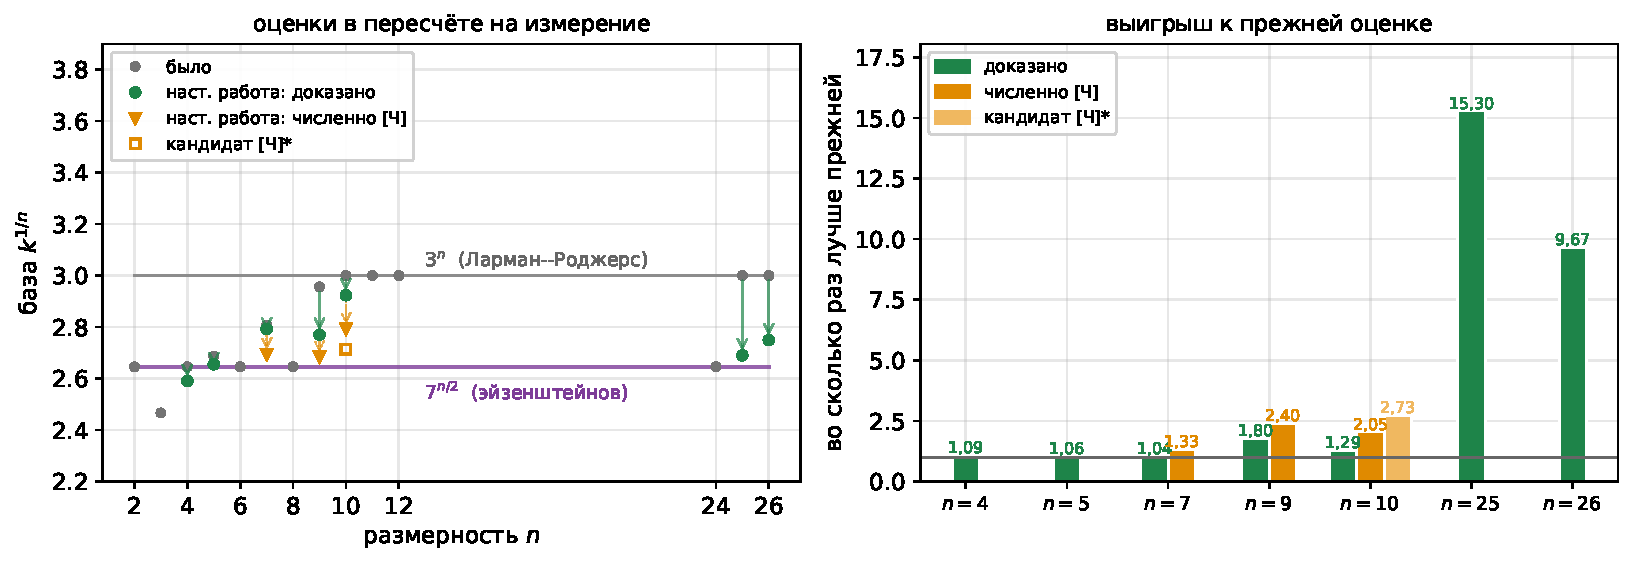
\includegraphics[width=\textwidth]{fig_landscape.pdf}
\caption{Слева: все известные верхние оценки в пересчёте на измерение,
$k^{1/n}$; горизонтали --- классический ориентир $3^n$ и эйзенштейнов $7^{n/2}$.
Стрелки показывают вклад настоящей работы. Видно, что размерности $8$ и $24$
достигают эйзенштейновой линии, а размерность~$10$ впервые уходит ниже
классической. Справа: выигрыш к прежней оценке.}
\label{fig:landscape}
\end{figure}

Верхняя оценка в размерности~4 имеет историю: $\le54$ (Радоичич, Тот
\cite{RadoicicToth}, решётка $A_4^*$); оценка $\le49$ заявлена без доказательства
Кулсоном и приведена в \cite{CoulsonPayne2007}; полное доказательство, вместе с
проверкой минимальности индекса~$49$ \emph{для решётки $D_4$}, дано Арманом,
Бондаренко, Прымаком и Радченко \cite{ABPR} (далее --- АБПР). Нижняя граница в
этой размерности прошла путь $6$ (Райский) $\to7$ \cite{Ivanov2006}
$\to9$ \cite{ExooIsmailescu}. В работе~\cite{ABPR} (открытый вопрос~1) высказано ожидание, что улучшить $49$
нельзя:
\begin{quote}\itshape\small
<<We believe that the answer is negative for $n=4,5$, i.e.
$\min\chi_s(\E^4,\Lambda,\Lambda',\ell)=49$~\ldots>> (\cite{ABPR}, Open
question~1),
\end{quote}
где минимум берётся по всем решёткам $\Lambda$, подрешёткам $\Lambda'$ и всем
$\ell>0$. Настоящая работа опровергает это ожидание.

\subsection{Результаты}

\begin{keybox}
\textbf{Основные результаты.} $\chi(\R^4)\le 45$; точнее,
$\chi\bigl(\R^4,[1,\ell]\bigr)\le45$ при всех $\ell\le1{,}015$
(теорема~\ref{thm:main}). Раскраска решёточная, задаётся явной рациональной
решёткой общего положения; ключевое неравенство доказано в точной рациональной
арифметике (\S\ref{sec:comp}). Кроме того,
$\chi\bigl(\R^5,[1,\ell]\bigr)\le132$ при $\ell\le1{,}01$, в частности
$\chi(\R^5)\le132$ (теорема~\ref{thm:r5}), и
$\chi\bigl(\R^7,[1,\ell]\bigr)\le1323$ при $\ell\le1{,}007$, в частности
$\chi(\R^7)\le1323$ (теорема~\ref{thm:r7}); обе новые конструкции имеют
рациональные компьютерно проверяемые сертификаты.

Ламинирование с \emph{кусочным сертификатом диаметра} (\S\ref{sec:dim912},
\S\ref{ssec:dim10lam}) даёт дополнительно $\chi(\R^7)\le1029$,
$\chi(\R^9)\le7203$ и $\chi(\R^{10})\le28812$ --- статус \textbf{[Ч]} (вся
плавающая точка сведена к значениям явных квадратик в вершинах явных
политопов; рационализация --- ближайшая задача).
\end{keybox}

\noindent Кроме того:
\begin{itemize}[leftmargin=1.4em,itemsep=1pt]
\item раскраска в $48$ цветов, правильная для более широкого интервала
$\ell\le1{,}0396$ (\S\ref{sec:wide}), --- компромисс <<меньше цветов ${}\leftrightarrow{}$
шире интервал>>, ранее не отмечавшийся;
\item точные ширины запрещённых интервалов \emph{всех} явных конструкций АБПР в
размерностях $4\le n\le9$ (\S\ref{sec:extra}; в \cite{ABPR} доказывалось лишь
$\ge1$), и тождество $D=\sqrt{7/3}\,\lambda_1$ для эйзенштейновых конструкций,
дающее их точную ширину и явно реализующее усиление из замечания~9
работы~\cite{ABPR};
\item уточнение (в большую сторону) нашей прежней таблицы \cite{Ivanov2011}
для $\R^3$ и исправление трёх допущенных в ней опечаток; кроме того, точный
сертификат $\chi(\R^3,[1,\ell])\le15$ при $\ell\le1{,}026$ и замкнутые формы
ширины в однопараметрическом семействе вокруг конструкции Кулсона, у которой
ширина равна ровно~$1$ (\S\ref{sec:stair});
\item масштабируемый метод поиска раскрасок для $n\ge5$: точное исправление
детерминанта по кофактору, CSP и min-conflicts, доводка по активному набору с доверительной областью, температурное продолжение метрики и безвершинное вычисление радиуса покрытия
(\S\ref{sec:big});
\item полный поиск по примарным CRT-блокам, пороговое расширение портфеля
дискретных бассейнов и дискретно-непрерывное чередование ядра и формы Грама,
понижающие оценку для $\R^5$ с $140$ до $132$ и опровергающие прежнюю
диагностику <<неустранимого>> единичного конфликта;
\item примарный Radon/FFT-поиск по полным блокам характеров конечных полей и
геометрически взвешенная целевая функция, которые совместно с деформацией формы
Грама понижают оценку в $\R^7$ с $1372$ до $1323$; прежние отрицательные
эксперименты на фиксированной $E_7^*$ объясняют, почему необходимы обе стадии
(\S\ref{sec:big});
\item лестницы ширин в $\R^5$ и $\R^6$ (табл.~\ref{tab:stair56}) и
воспроизводимые отрицательные экраны ближайших индексов в размерностях
$5$--$9$, не трактуемые как доказательства невозможности;
\item объёмный экран Минковского (предложение~\ref{prop:mink}) --- строгая
нижняя граница индекса для каждой родительской решётки, полученная без всякого
перебора, и диагностика, указавшая на размерность~$9$;
\item \emph{ламинирование} (\S\ref{sec:dim912}): подъём раскраски $\R^{n-1}$
слоями, опирающийся на две одностроч\-ные леммы; отсюда цепочка
$\chi(\R^9)\le17253\to9604\to7203$ и лестница ширин в $\R^9$, стремящаяся к
$\sqrt{7/6}$ --- ширине конструкции $E_8/2401$, а в размерности~$7$ ---
$\chi(\R^7)\le1029$ (ламинирование $E_6^*/343$, \S\ref{ssec:dim7});
\item \emph{продуктовое исчисление ширин} (предложение~\ref{prop:product}):
условие допустимости ортогонального произведения сворачивается в одно
неравенство $\sum_i 1/d_i^2\le1$ по одним лишь ширинам, с
$\ell=(\sum_i 1/d_i^2)^{-1/2}$; прежнее $\sum_i\rho_i^2\le4$ --- его частный
случай, а существенно то, что блоки могут иметь разный индекс. Отсюда
$\chi(\R^{10},[1,\sqrt{217/214}])\le2401\cdot19=45619$
(теорема~\ref{thm:dim10}) и оценки в размерностях $25$, $26$, а также
\emph{теорема о бюджете слоя} (предложение~\ref{prop:layerbudget}):
избыток ширины базы есть в точности бюджет радиуса покрытия на дополнительные
измерения;
\item \emph{слоевое ламинирование с двумерным слоем} (\S\ref{ssec:dim10lam}):
слои $A_2$ сдвигаются внутрь ячейки $E_8$ эквивариантными поправками, а
сертификат диаметра сводится редукцией к уже построенному двухслойному;
отсюда $\chi(\R^{10},[1,1{,}0432])\le28812$ --- лучше $3^{10}$ в $2{,}05$
раза;
\item \emph{инрадиусный экран индекса} (предложение~\ref{prop:inrfloor}) ---
второй строгий пол, не следующий из объёмного; вместе они запрещают плоский
блок индекса $\le16$ рядом с $E_8/2401$;
\item \emph{кусочный сертификат диаметра} (\S\ref{ssec:cert}): конечное общее
измельчение двух сдвинутых разбиений Вороного превращает верхнюю границу
радиуса покрытия слоёной решётки в конечный максимум выпуклых квадратик по
вершинам явных политопов --- сертификат откалиброван на точно известном
случае и закрывает главный пробел ламинирования;
\item \emph{планарная теорема} (предложение~\ref{prop:planar}):
$D((3+\omega)\Lambda)\ge\sqrt{7/3}\,\lambda_1$ для всех эйзенштейновых решёток
--- половина тождества~\eqref{eq:eis} доказана; как следствие, ширина
$\sqrt{7/6}$ для $\Lambda_{24}$ из гипотезы становится теоремой;
\item правило $D_{\min}(m\Lambda)=(m-1)\lambda_1$ для вещественного множителя
(предложение~\ref{prop:mult}, теперь с полным доказательством), инрадиусная
лемма~\ref{lem:inradius} со следствием о невозможности промежуточных подгрупп
при $\rho<2$, башня ламинаций $E_8$ при $n=10,11,12$ и ширина
$\sqrt{3/2}=1{,}2247$ при $n=12$ через решётку Коксетера--Тодда;
\item \emph{за пределами решёток} (\S\ref{sec:tilings}): класс раскрасок
периодическими степенными (лагерровыми) мозаиками, содержащий решёточную
схему как срез; пол $2^n$ для всего класса (теорема~\ref{thm:floor});
редукция к одной форме, объясняющая, почему в чемпионских индексах свобода
не окупается; точный учёт $k=F/\delta_C$ и окно $0{,}85\,\%$ эйзенштейновой
лестницы; и \emph{сертифицированные мозаичные ступени в плоскости}:
$\chi(\R^2,[1,\ell])\le8$ при $\ell\le1{,}4413$ и $\le15$ при
$\ell\le2{,}2815$ --- насколько нам известно, первые точные рациональные
сертификаты для нерешёточных мозаичных раскрасок (\S\ref{ssec:quant};
численно более сильные мозаики --- \cite{deGreyParts,Parts2023}); плюс
отрицательное: мозаичная свобода не понижает плоский проставок $19$, оценки
$\R^{10}$ устойчивы;
\item свободно доступная реализация всего конвейера (\S\ref{sec:algo}) с
многопоточным перебором и точной сертификацией.
\end{itemize}

\medskip\noindent
\textbf{Шкала статусов.} Работа сочетает доказательства, точные компьютерные
сертификаты и обширный численный поиск, поэтому всюду ниже утверждения
помечены одной из следующих меток:

\begin{description}[leftmargin=2.4em,itemsep=1pt,topsep=3pt]
\item[\textbf{[Т]}] \emph{теорема} --- доказано обычными средствами;
\item[\textbf{[С]}] \emph{точный сертификат} --- сведено к конечному набору
неравенств между рациональными числами, проверенных в точной арифметике дробей;
плавающая точка могла участвовать в \emph{выборе} кандидатов, но не в проверке;
\item[\textbf{[Ч]}] \emph{численный результат} --- получено вычислениями с
плавающей точкой; приводится как ориентир, доказательной силы не имеет;
\item[\textbf{[Ч]}${}^{*}$] \emph{кандидат} --- как \textbf{[Ч]}, но
сертификат диаметра отсутствует или находится на грани разрешения плавающей
точки; приводится как цель дальнейшей работы, а не как результат;
\item[\textbf{[Э]}] \emph{экран} --- перебор, завершившийся \emph{отрицательно}
и \emph{на фиксированной численной форме}. Экран не является доказательством
невозможности: изменение формы Грама выводит из перебранного множества.
\end{description}

\noindent Из оценок заголовка статус \textbf{[С]} имеют $45$ и $132$ (как и
промежуточная $1323$); оценки $1029$, $7203$ и $28812$ имеют статус
\textbf{[Ч]} --- их сертификаты диаметра выполнены в плавающей точке.
Подробное распределение статусов по утверждениям --- \S\ref{sec:origin}.


